\chapter{Simulation}
\label{sec:simulation}
In this chapter I discusses how particle physicists simulate high energy particle physics
interactions. Simulated interactions, based on knowledge of the Standard Model, provide 
the foundation of our predictions in high energy particle physics. 
The wealth of particle physics knowledge accumulated over the last 
60 years provides has provided a testing grounds to compare experimental results with
simulated particle interactions. Based on extensive work from the simulation community,
we are able to simulate and model the the proton-proton collisions which take place in the
CMS detector with a high degree of precision. Knowledge of what processes should take place
in our detector allows us to construct a prediction of what we will find. In the following
analyses, we are specifically interested in comparing two physics scenarios: the Standard Model 
without the existance of a 125 \GeV Higgs boson versus the Standard Model with the existance
of a 125 \GeV Higgs boson. Both of these predictions rely on the Standard Model processing and
Higgs boson processes be well modeled.
In this chapter, I specifically focus on how events are simulated for proton-proton collisions,
how the initial products of the collision decay, and how the decay products are modeled
to interact with a simulation of the CMS detector.


\section{Hard Scattering Process}
Monte Carlo Generator Programs
FSR ISR
    Resonance Decays

\section{Parton Distribution Functions}
One of the unique complexities present at a hadron collider which is avoided with a
lepton collider is accounting for the substructure of the colliding hadrons. For proper simulations
of LHC proton-proton collisions we must account for this. The internal structure of the proton
has been probed over the past half century using deep inelastic scattering~\cite{Breidenbach:1969kd, PhysRevLett.23.930}.
Experimental results showed the internal structure of protons revealing the existance of
quarks and gluons. The internal structure of the colliding protons at the LHC are taken into
account using what are called Parton Distribution Function (PDFs). PDFs give the probability
density for finding a particle a parton with a certain longitudinal momentum fraction $x$ at a given
energy scale. The momentum fraction $x$ is the the parton's fractional momentum with respect
to the hadron under consideration, protons for CMS related simulations. 
%Figure~\ref{fig:sim_pdf} 
%shows example PDFs for two given energy scales. 

The specific PDFs which are used in the
following analyses are provided by \texttt{NNPDF3.0} with the exact PDF set being 
\texttt{NNPDF30\_nlo\_as\_0118}~\cite{Ball:2014uwa, Ball:2011uy}. The \texttt{NNPDF3.0} PDFs
use a global dataset including, but not limited to, data from HERA, ZEUS, ATLAS, LHCb, and CMS.
Functional forms derived from theoretical QCD predictions with electroweak corrections are fit
to the available data resulting in the provided PDFs used by CMS for event simulation~\cite{Ball:2014uwa}.
Uncertainties from the PDF estimation method are applied in the following analyses to cover
potential mismodeling of the proton PDFs used in the CMS simulations.



\section{Underlying Event}
In addition to the particles resulting from the hard scattering portion of a proton-proton collision,
there is what is called the underlying event. The underlying event consists of interactions between
partons not directly associated with hard scattering event. This comes from interactions of 
secondary partons within the colliding protons which are not the two hard scatter partons.
The soft, low energy nature of the underlying event interactions limits the range of physics
processes which can result from their interactions. At this level in simulated event generation,
the most common underlying event interactions result in two partons interacting resulting in a 
single parton. This is only an intermediary stage as color confinement eliminates the possibility
of a single isolated parton propagating through the CMS detector, this will be revisited shortly.

The underlying event in 
Monte Carlo event generators predominantly characterize the kinematics and compostion of soft ``jets''.
There are specific ``jet'' related physics observabes which are sensitive to the characteristics of the underlying
event~\cite{Khachatryan:2015pea, Field:cdf2008}. For a description of ``jets'' see Section~\ref{sec:obj_reco_jets}.
The initial underlying event tune for \POWHEG 8 is the Monash Tune. A CMS specific tuning of 
\POWHEG 8 has been constructed using the parameters of the Monash Tune. The tune is based
on data from CDF and 7 \TeV CMS data and is called \texttt{CUETP8M1}. The differences between
\texttt{CUETP8M1} and the Monash Tune related to the treatement of the energy-dependence 
parameters in the fit. Considering \texttt{CUETP8M1} is derived based largely on data from
CMS, there is very good agreement between CMS data and simulations based on the
\texttt{CUETP8M1} tune~\cite{Khachatryan:2015pea}. 



\section{Parton Showers}
The next step in created simulated events deals with the partons resulting from ISR,
FSR, and the underlying event. 
While matrix elements are used to calculate the hard scattering event plus ISR and FSR, 
the use of matrix element to fully describe the production and decay of all of the
partons is technically not possible with current best Monte Carlo generators~\cite{PhysRevD.94.074005}. 
Instead, these partons are decayed using the parton shower method. 
Parton shower evolution can be viewed as a probabilistic process 
which occures with unit total probability where each produced parton has a probability
of radiating another parton. Partons iteratively decay through three 
dominant processes: $\textrm{q} \to \textrm{gq}$, $\textrm{g} \to \textrm{gg}$, 
and $\textrm{g} \to \textrm{q}\bar{\textrm{q}}$. 

Technically, there is a matching and merging of the hard scatter matrix element with the
parton shower contribution. This does not affect the total process cross section.
The Monte Carlo generators used in this thesis are interfaced with 
\PYTHIA 8.212~\cite{Sjostrand:2014zea} to model the parton shower evolution.



\section{Hadronization}
As mentioned previously, due to color confinement, quarks and gluons can not exist in isolation
and must be transformed in color-neutral final states~\cite{Hoche:2014rga}. 
To resolve the lone quarks and gluons which resulted from the hard scatter process and the parton 
shower, the partons undergo hadronization. Hadronization is the process where hadrons are formed 
out of quarks and gluons. There are multiple phenomenological models of hadronization, the
specific ones used in this thesis is the Lund String Model. The Lund String Model of jet
hadronization is based the observation that within a meson system the quark-antiquark 
potential rises linearly with the distance between quarks~\cite{Bali:1992ab}. In the model, this
potential energy is stored in flux lines connecting the quark-antiquark pair, see left pane 
Figure~\ref{fig:sim_lund_string}. As a quark-antiquark 
pair with high energy moves apart the energy stored between them in the flux lines increases. If the energy
is sufficiently high the flux line can be severed as a second quark-antiquark pair are created from
the freed energy. This can be visualized the right pane of Figure~\ref{fig:sim_lund_string}.
This process repeats itself creating stable mesons and baryons where the low energy (anti)quarks
oscillate about eachother, represented as the zig-zag lines in Figure~\ref{fig:sim_lund_string}.

\begin{figure*}[htbp]
\centering
     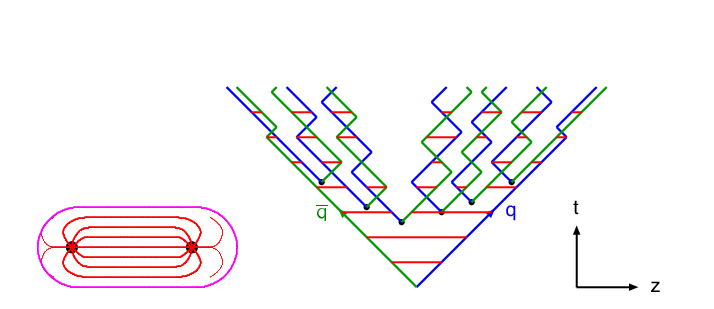
\includegraphics[width=0.7\textwidth]{simulation/plots/lund_time-space.png}
     \caption{
(left) Lund String Model flux tubes connecting a quark-antiquark pair. (right) A
space-time representation of the breakup of an original quark-antiquark pair with
excess energy. The final representation here depicts seven mesons.
     }
     \label{fig:sim_lund_string}
\end{figure*}



\section{Pileup}
There where 27 proton-proton collisions per bunch crossing on average
in the 2016 data collected by CMS.
For most bunch crossings all of these proton-proton collisions are soft
scattering events and, with no hard process present, the event it unlikely to be stored for
future physics analysis because it will fail the Level-1 or High Level Trigger selections. 
When there is a hard scattering process present in a bunch crossing,
these soft scattering collisions will still be present and must be modeled. 
To emulate this effect in simulated events, in addition to the two protons involved in the 
hard scattering interaction, additional proton-proton interactions are added. 
These additional proton-proton collisions are
dominated by the same type of soft scattering collisions observed in data and are referred to as ``pileup''.
\textsc{Pythia8} is used to generate these soft scattering collision. 
The distribution of the number of soft scattering events added to a simulated 
sample is intended to align with the distribution observed in the 2016 data.
As alignment is never 100\% perfect immediately after the samples are simulated, the simulated events
are weighted to adjust their distribution to the data based on the measured instantaneous
luminosity for each bunch crossing, see Section~\ref{sec:htt_mc_samples}.



\section{Detector Simulation}
At this stage of event simulation, the simulated events model our best approximation
of the proton-proton collisions and resulting decays and hadronization taking place
in the CMS detector. There is one critical last step to complete the event
simulations. The decay products from the collisions must interact with a simulated
model of the CMS detector. The result of this final stage is simulated events that
are stored in the same data format as the data gathered by the detector itself,
raw energy deposits.

The \textsc{Geant4} software toolkit is used to simulate the CMS 
detector~\cite{Agostinelli:2002hh}. At its most basic, \textsc{Geant4} is a 
toolkit for simulating the passage of particles through matter. It contains a 
vast library of functionality allowing the creation of model physics detectors
made out of any desired material and in any desired geometrical configuration.
To validate the \textsc{Geant4} modeling of the CMS detector, test beam data and
collision data are used. Good agreement is seen between the data and the
simulated particles passing through the CMS detector for the energy response
and resolution for pions and protons~\cite{geant4_cms_2017}.

After the decay products of the simulated events have passed through the \textsc{Geant4}
simulation, they are stored in the same format as data is originally gathered. From
this point forward, data and simulated events are reconstructed with the same 
algorithms.




Signal and background processes are modeled with samples of simulated events.
The signal samples with a Higgs boson produced through gluon fusion ($\cPg\cPg\PH$), vector boson fusion (VBF),
or in association with a $\PW$ or $\PZ$ boson ($\PW\PH$ or $\PZ\PH$), are generated at next-to-leading order (NLO) in perturbative quantum chromodynamics (pQCD) with the \POWHEG 2.0~\cite{Nason:2004rx,Frixione:2007vw, Alioli:2010xd, Alioli:2010xa, Alioli:2008tz} generator. The \textsc{minlo hvJ}~\cite{Luisoni:2013kna} extension of \POWHEG 2.0 is used for the $\PW\PH$ and $\PZ\PH$ simulated samples. 
The $\ttbar\PH$ process is negligible.
The various production cross sections and branching fractions for the SM Higgs boson production, and their corresponding uncertainties are taken from Refs.~\cite{deFlorian:2016spz,Denner:2011mq,Ball:2011mu} and references therein.

The \aMCATNLO~\cite{Alwall:2014hca} generator is used for $\PZ+$jets and $\PW+$jets processes. They are simulated at leading order (LO) with the MLM jet matching and merging~\cite{Alwall:2007fs}.
The \aMCATNLO generator is also used for diboson production simulated at next-to-LO (NLO) with the FxFx jet matching and merging~\cite{Frederix:2012ps}, whereas \POWHEG 2.0 and 1.0 are used for $\ttbar$ and single top quark production, respectively.



